%%%%%%%%%%%%%%%%%%%%%%%%%%%%%%%%%%%%%%%%%
% Template LaTeX Template Version 1.0 (December 8 2014)
%
% This template has been downloaded from: http://www.LaTeXTemplates.com
%
% Original author: Brandon Fryslie With extensive modifications by: Vel
% (vel@latextemplates.com)
%
% License: CC BY-NC-SA 3.0 (http://creativecommons.org/licenses/by-nc-sa/3.0/)
%
% Authors: Sabbir Ahmed, Jeffrey Osazuwa, Howard To, Brian Weber
% 
%%%%%%%%%%%%%%%%%%%%%%%%%%%%%%%%%%%%%%%%%

\documentclass[paper=usletter, fontsize=12pt]{article}
\usepackage{graphicx}
%%%%%%%%%%%%%%%%%%%%%%%%%%%%%%%%%%%%%%%%%
% Structure
% Structural Definitions File
% Version 1.0 (December 8 2014)
%
% Created by:
% Vel (vel@latextemplates.com)
% 
% This file has been downloaded from:
% http://www.LaTeXTemplates.com
%
% License:
% CC BY-NC-SA 3.0 (http://creativecommons.org/licenses/by-nc-sa/3.0/)
%
%%%%%%%%%%%%%%%%%%%%%%%%%%%%%%%%%%%%%%%%%

\usepackage{geometry} % Required to modify the page layout

\usepackage{amsmath}
\usepackage{amssymb}

\usepackage[utf8]{inputenc} % Required for including letters with accents
\usepackage[T1]{fontenc} % Use 8-bit encoding that has 256 glyphs

\usepackage{avant} % Use the Avantgarde font for headings
\usepackage{setspace}

\setlength{\parindent}{0mm} % Don't indent paragraphs
\setlength{\parskip}{2.5mm} % Whitespace between paragraphs

\setlength{\textwidth}{16cm} % Width of the text on the page
\setlength{\textheight}{23cm} % Height of the text on the page
\setlength{\oddsidemargin}{0cm} % Width of the margin - negative to move text left, positive to move it right
\setlength{\topmargin}{-1.25cm} % Reduce the top margin

\renewcommand\familydefault{\sfdefault}  % default font for entire document
 % specifies the document layout and style

%----------------------------------------------------------------------------------------

% names
\newcommand{\team}{Galois Field Arithmetic Unit}
\newcommand{\Sabbir}{Sabbir Ahmed}
\newcommand{\Jeffrey}{Jeffrey Osazuwa}
\newcommand{\Howard}{Howard To}
\newcommand{\Brian}{Brian Weber}

% document info command
\newcommand{\documentinfo}[5]{
    \begin{centering}
        \parbox{6.8in}{
        \begin{spacing}{1}
            \begin{flushleft}
                \begin{tabular}{l l} #1 \\ #2 \\ #3 \\ #4 \\ #5 \\
                \end{tabular}\\
                \rule{\textwidth}{1pt}
            \end{flushleft}
        \end{spacing} }
    \end{centering} }

\begin{document}

    \documentinfo {\textbf{MEMO NUMBER:} GFAU-SOW} {\textbf{DATE:} {\today}}
    {\textbf{TO: } EFC LaBerge} {\textbf{FROM: }\Sabbir, \Jeffrey, \Howard,
    \Brian} {\textbf{SUBJECT: } Galois Field Arithmetic Unit Statement of Work}
    \vspace{-0.3in}

    \section{Introduction} A Galois field is a field with a finite number of
    elements. The nomenclature $GF(q)$ is used to indicate a Galois field with
    q elements. For $GF(q)$ in general, $q$ must be a power of a prime. For
    each prime power, there exists exactly one finite field. The best known and
    most used Galois field is $GF(2)$, the binary field.

    The \team~ handles irreducible polynomials in $GF(2^n)$, where $\{2 \leq n
    \leq 16\}$. The ALU generates all the terms in the field of the polynomial,
    and allows the user to view and apply the following binary operations:

    \begin{itemize}

        \item Addition
        \item Subtraction
        \item Multiplication
        \item Division
        \item Logarithm

    \end{itemize}

        \subsection{Purpose and Scope} This Statement of Work outlines and
        elaborates the tasks necessary to implement the project. The document
        also details their corresponding milestones and deadlines and how the
        contribution will be divided within the team.

    \section{Roles and Division of Labor} This project requires equal team work
on all tasks because of the steep learning curve on implementing coprocessors
with programmable boards. None of the team members have comprehensive prior
knowledge or training on field programmable gate array units, and are therefore
required to learn the concepts concurrently.

Although there is no clear division of labor within the team, each members have been implicitly designated unofficial roles.

Howard has been chosen to act as the point of contact between the team and the project manager and other consultants. He has also been trusted with the scheduling of team meetings and milestones.

Sabbir is responsible for validating the system inputs and outputs through the operations in the unit. He is also accountable for providing background information on the Galois field and its operations related to the arithmetic unit.

Brian has been put in charge with the digital design of the system at various levels. He is also responsible for overseeing the designing of the system using the hardware description language.

Jeffrey supports the designing processes by providing test benches and by synthesizing the individual modules.

Each members of the GFAU shall contribute to designing the individual modules and the entire system.

    \section{Tasks}

        \subsection{Research}In this section, we introduce a series of questions that shall be answered in our preliminary research relating to the title of each subsection.

        \subsubsection{Background}The team shall conduct extensive research on the mathematics and theoretical concepts behind the operations in the GFAU. The unit emphasizes on the terms and the unary and binary operations among them bounded in the Galois field. A strong understanding on such topics is therefore essential for successful and accurate computations. 
        \subsubsection{Devices}The team shall conduct extensive research on the implementation and synthesis of digital design on programmable boards and their corresponding best practices. 
        

            \paragraph{Field Programmable Gate Array (FPGA)}What are designs that are commonly used, such as common arithmetic operations that will be helpful in the design of our system? What is and isn't allowed in VHDL in order for it to be synthesizable? What are some important specifications to look at when shopping for an FPGA? What are specifications do we need of our FPGA to meet our requirements?

            \paragraph{External Devices}What are some external devices that we will need to use? How will the GFAU communicate with these devices? What specifications are required of these devices to meet our system requirements?

        \subsection{Design}

            \subsubsection{System Boundary}A system boundary diagram detailing the functions, inputs and outputs of our system shall be developed. Additional diagrams elaborating on various hierarchies or the project shall also be developed, including the functional flow and data flow diagrams.

            \subsubsection{Schematics}Several schematics for the project may be developed and utilized during the development phase. A high-level schematic consisting of all the modules in the system shall be developed for the final product. The schematic shall be divided into segments to be elaborated on a lower level by individual members.

        \subsection{Software Implementation}

            \subsubsection{Design in VHSIC Hardware Description Language (VHDL)}Each of the operations in the GFAU: addition, subtraction, multiplication, division and logarithm, shall be implemented with independent and discrete VHDL modules. The source code shall be written and comprehensively documented using the best practices and standards imposed by the "IEEE Standard VHDL Language Reference Manual".

            \subsubsection{Simulation and Synthesis in VHDL}In order to ensure that the source code is functional, testing shall be performed after the completion of each module The modules shall be completed using standards for synthesis. Each modules shall be independently synthesized to ensure they match the intended schematics and designs. All simulations and software testing are expected to be completed by the end of November. 

            \subsubsection{External Devices}External devices such as memory may be required in our project. Should they be needed, their behavior shall be abstracted in VHDL so we can integrate and test our code to make sure it will work with the external devices. Any code written to describe the behavior of external devices does not have to be synthesizable, however. 

        \subsection{Purchases}An external memory chip suitable for storing the lookup tables created during the polynomial term generation shall be researched extensively before purchase. Research on the external memory interface includes simulation and testing of its truth tables using VHDL. A development board shall be researched on concurrently before being purchased for prototyping the implementation. The board shall comply with the constraints detailed in the System Requirement Specifications. 

        \subsection{Hardware}

            \subsubsection{Integration}The system shall be integrated with an FPGA board bounded by the constraints detained in the Systems Requirement Specifications. The board shall successfully communicate with a microcontroller for user interface and its external memories. The hardware integration shall be completed by mid-semester during spring after all purchases are made final.
            \subsubsection{Hardware Testing}Extensive testing on the FPGA board and its external components shall be conducted before, during and after the integration with the VHDL system modules. The testing of the hardware in the system shall server as the final milestone for the project during the end of the spring semester. 

    \section{Deliverables}Table 1 detail the expected deliverables throughout the project and shall be completed concurrently with the project development:

   \begin{table}[h]
   \caption{Expected Deliverable}
    
 \begin{center}
 	
    \begin{tabular}{ | p{5cm} | p{7cm} | l | p{5cm} |}
    
    \hline
    
    Deliverable & Description & Deadline \\ \hline
    System Specification Requirements & A detailed specification of the unit shall be developed including both hardware and software requirements, and any of the constraints that needed to be met. The System Specification Requirements also detailed all the inputs and outputs of the GFAU. & October 18, 2017
    \\ \hline
   Weekly Team Status Reports & Weekly status reports by the GFAU team shall be submitted to Dr. LaBerge discussing the completed tasks and issues encountered for the current period. They shall also include planned tasks for the next period & Weekly\\ \hline
    Preliminary Design Review & A Preliminary Design Review of the project shall be reviewed by Dr. LaBerge in the first week of December. & First week of December \\ \hline
    
    Completed Design Review & A final review of the GFAU shall be reviewed by Dr. LaBerge in May, 2018. & May, 2018 \\ \hline
    
    Demo & A fully functional GFAU shall be presented in May, 2018 to Dr. LaBerge. & May, 2018 \\ \hline
    \end{tabular}
    
\end{center}
\end{table}
\newpage
\section{Timeline}Figure 1 below shows a timeline of the capstone project in a Gantt Chart. \\

\begin{figure}[h]
	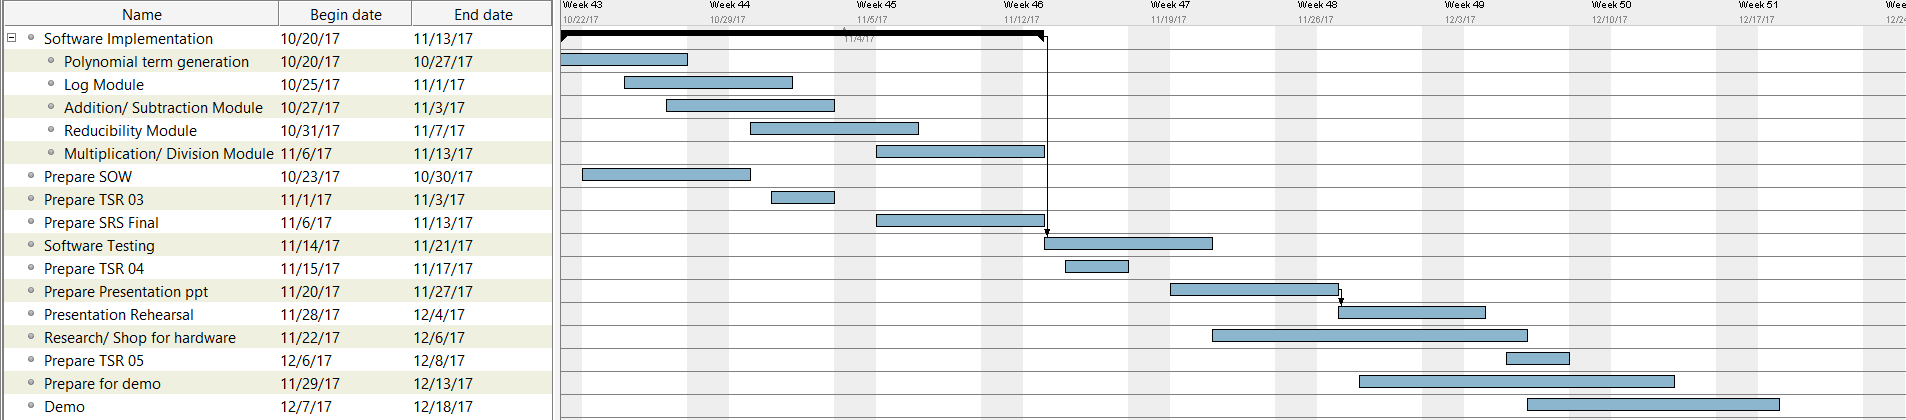
\includegraphics[scale=0.45]{gnatt_chart}
	\caption{Capstone schedule}

\end{figure}


\end{document}
